%%% LaTeX Template: Two column article
%%%
%%% Source: http://www.howtotex.com/
%%% Feel free to distribute this template, but please keep to referal to http://www.howtotex.com/ here.
%%% Date: February 2011

%%% Preamble
\documentclass[	DIV=calc,%
							paper=a4,%
							fontsize=11pt]{scrartcl}	 					% KOMA-article class

\usepackage[spanish]{babel}										% English language/hyphenation
\usepackage[protrusion=true,expansion=true]{microtype}				% Better typography
\usepackage{amsmath,amsfonts,amsthm}					% Math packages
%\usepackage[pdftex]{graphicx}									% Enable pdflatex
\usepackage[svgnames]{xcolor}									% Enabling colors by their 'svgnames'
\usepackage[hang, small,labelfont=bf,up,textfont=it,up]{caption}	% Custom captions under/above floats
\usepackage{epstopdf}												% Converts .eps to .pdf
\usepackage{subfig}													% Subfigures
\usepackage{booktabs}												% Nicer tables
\usepackage{fix-cm}													% Custom fontsizes
\usepackage{hyperref}

\usepackage[T1]{fontenc}
\usepackage[utf8]{inputenc}
\usepackage[light]{kurier}


%%% Custom sectioning (sectsty package)
\usepackage{sectsty}													% Custom sectioning (see below)
\allsectionsfont{%															% Change font of al section commands
	\usefont{T1}{mdugm}{b}{it}%										% bch-b-n: CharterBT-Bold font
	}

\sectionfont{%																% Change font of \section command
	\usefont{T1}{mdugm}{b}{it}%										% bch-b-n: CharterBT-Bold font
	}

%%% Headers and footers
\usepackage{fancyhdr}												% Needed to define custom headers/footers
	\pagestyle{fancy}														% Enabling the custom headers/footers
\usepackage{lastpage}

% Header (empty)
\lhead{}
\chead{}
\rhead{}
% Footer (you may change this to your own needs)
\lfoot{\footnotesize \miit{Alejandro Alcalde, Cristina Heredia} \textbullet ~}
\cfoot{}
\rfoot{\footnotesize Página \thepage\ de \pageref{LastPage}}	% "Page 1 of 2"
\renewcommand{\headrulewidth}{0.0pt}
\renewcommand{\footrulewidth}{0.4pt}



%%% Creating an initial of the very first character of the content
\usepackage{lettrine}
\newcommand{\initial}[1]{%
     \lettrine[lines=3,lhang=0.3,nindent=0em]{
     				\color{DarkGoldenrod}
     				{\textsf{#1}}}{}}



%%% Title, author and date metadata
\usepackage{titling}															% For custom titles

\newcommand{\HorRule}{\color{DarkGoldenrod}%			% Creating a horizontal rule
									  	\rule{\linewidth}{1pt}%
										}

\pretitle{\vspace{-30pt} \begin{flushleft} \HorRule
				\fontsize{50}{50} \usefont{T1}{kurier}{l}{it} \color{DarkRed} \selectfont
				}
\title{NPI P3: Android}					% Title of your article goes here
\posttitle{\par\end{flushleft}\vskip 0.5em}

\preauthor{\begin{flushleft}
					\large \lineskip 0.5em \usefont{T1}{mdugm}{m}{it} \color{DarkRed}}
\author{Cristina Heredia, Alejandro Alcalde,\;}											% Author name goes here
\postauthor{\footnotesize \usefont{OT1}{mdugm}{m}{it} \color{Black}
					Universidad de Granada 								% Institution of author
					\par\end{flushleft}\HorRule}

\date{\usefont{T1}{mdugm}{b}{it}\selectfont\today}																				% No date

\newcommand{\miit}[1]{{\usefont{T1}{mdugm}{m}{it}\selectfont #1}}

\usepackage[nottoc]{tocbibind}

\usepackage[outputdir=metafiles]{minted}

\newminted{java}{
		numbersep=5pt,
		autogobble=true,
		frame=lines,
		framesep=2mm,
		fontsize=\scriptsize,
		tabsize=2,
		fontfamily=DejaVuSansMono-TLF,
		breaklines,
}
\newminted{xml}{
		numbersep=5pt,
		autogobble=true,
		frame=lines,
		framesep=2mm,
		fontsize=\scriptsize,
		tabsize=2,
		fontfamily=DejaVuSansMono-TLF,
		breaklines,
}

\newmintinline{java}{fontsize=\scriptsize, fontfamily=DejaVuSansMono-TLF}
\newmintinline{xml}{fontsize=\scriptsize, fontfamily=DejaVuSansMono-TLF}

\usepackage{graphicx}

%%% Begin document
\begin{document}
\maketitle
\tableofcontents
\thispagestyle{fancy} 			% Enabling the custom headers/footers for the first page
% The first character should be within \initial{}
%

\section{Tutoriales de las aplicaciones
Android}\label{tutoriales-de-las-aplicaciones-android}

\subsection{BrujulaCompass}\label{brujulacompass}

Para realizar esta aplicación se ha tomado como base la brújula de la
\emph{ROM} MIUI. Se le ha añadido el reconocimiento de voz (\emph{ASR})
y se modificó la la interfaz de la brújula para que mostrara hacia donde
tiene que dirigirse el usuario en función del comando de voz. Veamos la
primera pantalla:

\subsubsection{Inicio de la
aplicación}\label{inicio-de-la-aplicaciuxf3n}

\begin{figure}[H]
\centering
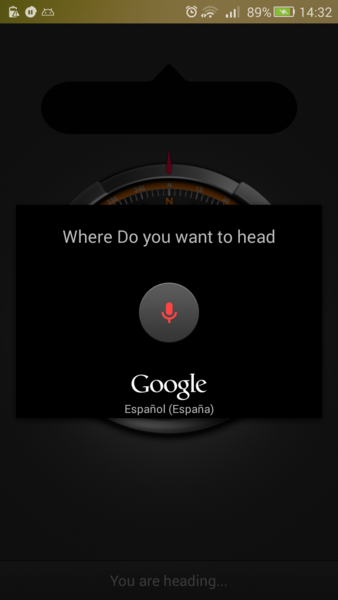
\includegraphics[width=0.5\textwidth]{./img/inicioBrujula.png}
\caption{Primera pantalla de la aplicación brújula}
\end{figure}

Al mostrarse esta pantalla, el usuario debe proporcionar un comando de
voz, por ejemplo \emph{``Norte 10''}. Tras dar el comando, en la brujula
se añadirá un marcador indicando dónde está el Norte + 10 grados. Además
de esto, mediante una voz, se le irá indicando al usuario si debe girar
a la derecha/izquierda o va en la dirección correcta:

\begin{figure}[H]
\centering
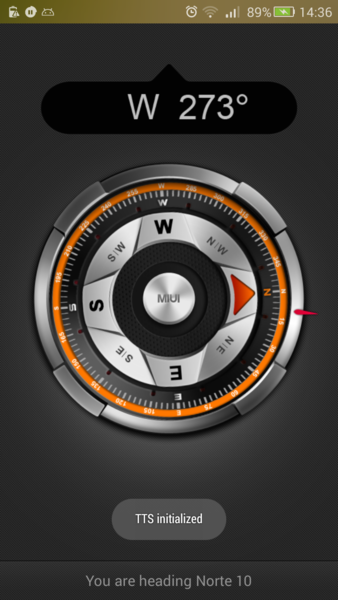
\includegraphics[width=0.5\textwidth]{./img/norte10.png}
\caption{Indicaciones en la brujula}
\end{figure}

Como vemos en la imagen, aparece un indicador rojo situado en el norte +
10 grados. Veamos otro ejemplo, Norte 45:

\begin{figure}[H]
\centering
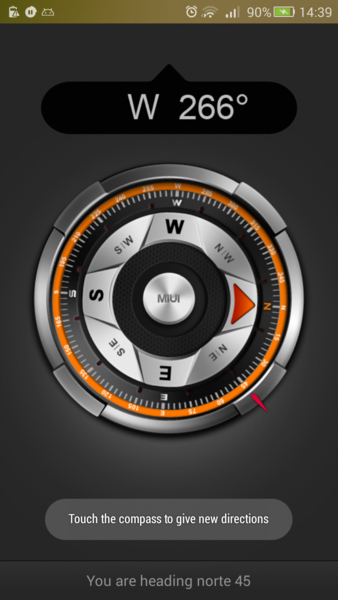
\includegraphics[width=0.5\textwidth]{./img/norte45.png}
\caption{Indicaciones en la brujula}
\end{figure}

Para dar nuevas instrucciones de voz basta con tocar la brújula.

En la parte inferior de la pantalla, aparece el comando de voz
reconocido.

\subsubsection{Implementación}\label{implementaciuxf3n}

Se han necesitado de tres clases, La principal que implementa la
actividad (\texttt{CompassActivity}), donde reside prácticamente toda la
lógica de la aplicación. En ella se hace uso de los sensores magnético y
el acelerómetro. La otra clase ha es una extensión de la clase
\texttt{ImageVew} para crear nuestra propia vista, en este caso el
compás y el indicador de la dirección indicada por el usuario.

\paragraph{Clase CompassActivity.java}\label{clase-compassactivity.java}

Esta clase es la principal y en la que se realiza toda la lógica, en
ella se declarar y registran los sensores a usar (El magnético y el
acelerómetro). Ambos se obtienen en el método \texttt{onCreate} del
siguiente modo:

\begin{javacode}
	private SensorManager mSensorManager;
	private Sensor mMagneticSensor;
	private Sensor mAccelerometer;

	//...

	mSensorManager = (SensorManager) getSystemService(Context.SENSOR_SERVICE);
	mMagneticSensor = mSensorManager.getDefaultSensor(Sensor.TYPE_MAGNETIC_FIELD);
	mAccelerometer = mSensorManager.getDefaultSensor(Sensor.TYPE_ACCELEROMETER);
\end{javacode}

Para poder obtener actualizaciones frecuentes de los datos de los
sensores es necesario declarar un \texttt{SensorEventListener} y
registrarlo en el sistema, declararemos un único \emph{listener} que
será usado por los dos sensores:

\begin{javacode}
	private SensorEventListener mMagneticSensorEventListener = new SensorEventListener() {

			@Override
			public void onSensorChanged(SensorEvent event) {

					if (event.sensor == mMagneticSensor) {
							System.arraycopy(event.values, 0, mLastMagnetometer, 0, event.values.length);
							mLastMagnetometerSet = true;
					} else if (event.sensor == mAccelerometer) {
							System.arraycopy(event.values, 0, mLastAccelerometer, 0, event.values.length);
							mLastAccelerometerSet = true;
					}

					if (mLastAccelerometerSet && mLastMagnetometerSet) {
							SensorManager.getRotationMatrix(mR, null, mLastAccelerometer, mLastMagnetometer);
							SensorManager.getOrientation(mR, mOrientation);
							float azimuthInRadians = mOrientation[0];
							float azimuthInDegress = (float) (Math.toDegrees(azimuthInRadians) + 360) % 360;

							mTargetDirection = -azimuthInDegress;
					}
			}

			@Override
			public void onAccuracyChanged(Sensor sensor, int accuracy) {
			}
	};
\end{javacode}

La función \texttt{onSensorChanged} será llamada cada vez que se
actualicen los datos de los sensores.

Una vez tenemos una referencia a los sensores y el \emph{listener}
creado, hay que registrarlos en el método \texttt{onResume} y
des-registrarlos en el \texttt{onPause}:

\begin{javacode}
	@Override
	protected void onResume() {
			super.onResume();

			if (mMagneticSensor != null) {
					mSensorManager.registerListener(mMagneticSensorEventListener, mMagneticSensor,
									SensorManager.SENSOR_DELAY_GAME);
			}
			if (mAccelerometer != null) {
					mSensorManager.registerListener(mMagneticSensorEventListener, mAccelerometer,
									SensorManager.SENSOR_DELAY_GAME);
			}
			// ...
	}

	@Override
	protected void onPause() {
			super.onPause();

			if (mMagneticSensor != null) {
					mSensorManager.unregisterListener(mMagneticSensorEventListener);
			}
			if (mAccelerometer != null) {
					mSensorManager.unregisterListener(mMagneticSensorEventListener);
			}

			// ...
	}
\end{javacode}

El reconocimiento de voz se inicializa en el siguiente método:

\begin{javacode}
	/**
	 * Starts listening for any user input.
	 * When it recognizes something, the <code>processAsrResult</code> method is invoked.
	 * If there is any error, the <code>processAsrError</code> method is invoked.
	 */
	private void startListening() {
			Intent intent = new Intent(RecognizerIntent.ACTION_RECOGNIZE_SPEECH);
			intent.putExtra(RecognizerIntent.EXTRA_LANGUAGE_MODEL, RecognizerIntent.LANGUAGE_MODEL_FREE_FORM);
			intent.putExtra(RecognizerIntent.EXTRA_PROMPT, getString(R.string.asr_prompt));
			intent.putExtra(RecognizerIntent.EXTRA_MAX_RESULTS, 2);

			try {
					startActivityForResult(intent, REQUEST_RECOGNIZE);
			} catch (ActivityNotFoundException e) {
					//If no recognizer exists, download from Google Play
					showDownloadDialog();
			}
	}
\end{javacode}

Esto intentará lanzar el reconocedor de voz, si el dispositivo no lo
tiene instalado lanzará un diálogo pidiendo al usuario que lo instale:

\begin{javacode}
	private void showDownloadDialog() {
			AlertDialog.Builder builder =
							new AlertDialog.Builder(this);
			builder.setTitle(R.string.asr_download_title);
			builder.setMessage(R.string.asr_download_msg);
			builder.setPositiveButton(android.R.string.yes,
							new DialogInterface.OnClickListener() {
									@Override
									public void onClick(DialogInterface dialog,
																			int which) {
											//Download, for example, Google Voice Search
											Intent marketIntent =
															new Intent(Intent.ACTION_VIEW);
											marketIntent.setData(
															Uri.parse("market://details?"
																			+ "id=com.google.android.voicesearch"));
									}
							});
			builder.setNegativeButton(android.R.string.no, null);
			builder.create().show();
	}
\end{javacode}

Una vez que el usuario habla, se recoge el resultado en el
\texttt{onActivityResult} y decidimos cómo interpretarlo, en este caso
se parsea de forma bastante primitiva si el usuario dijo \emph{este,
norte, sur u oeste} junto al número de grados:

\begin{javacode}
	@Override
	protected void onActivityResult(int requestCode, int resultCode, Intent data) {
			if (requestCode == REQUEST_RECOGNIZE &&
							resultCode == Activity.RESULT_OK) {
					ArrayList<String> matches =
									data.getStringArrayListExtra(RecognizerIntent.EXTRA_RESULTS);

					String[] tokens = matches.get(0).split(" ");

					if (tokens.length == 2) {
							mHeadedDirection = Float.parseFloat(tokens[1]);
							mLocationTextView.setText(String.format(getString(R.string.heading_text), matches.get(0)));

							switch (tokens[0].toLowerCase()) {
									case "este":
											mHeadedDirection += 90;
											break;
									case "sur":
									case "surf":
											mHeadedDirection += 180;
											break;
									case "oeste":
											mHeadedDirection += 270;
											break;
							}

							Toast.makeText(this, R.string.asr_ask_again,
											Toast.LENGTH_LONG).show();

					} else {
							Toast.makeText(this, R.string.asr_error,
											Toast.LENGTH_LONG).show();
					}
			}
	}
\end{javacode}

El punto cardinal junto con los grados servirán para situar el indicador
que muestre al usuario hacia dónde debe dirigirse.

Para lograr el efecto de giro de la brújula, se rota la imagen con cada
actualización de los sensores:

\begin{javacode}
	protected Runnable mCompassViewUpdater = new Runnable() {
			@Override
			public void run() {
					if (mPointer != null && !mStopDrawing) {
							if (mDirection != mTargetDirection) {

									// calculate the short routine
									float to = mTargetDirection;
									if (to - mDirection > 180) {
											to -= 360;
									} else if (to - mDirection < -180) {
											to += 360;
									}

									// limit the max speed to MAX_ROTATE_DEGREE
									float distance = to - mDirection;
									float MAX_ROATE_DEGREE = 1.0f;
									if (Math.abs(distance) > MAX_ROATE_DEGREE) {
											distance = distance > 0 ? MAX_ROATE_DEGREE : (-1.0f * MAX_ROATE_DEGREE);
									}

									// need to slow down if the distance is short
									mDirection = normalizeDegree(mDirection
													+ ((to - mDirection) * mInterpolator.getInterpolation(Math
													.abs(distance) > MAX_ROATE_DEGREE ? 0.4f : 0.3f)));
									mPointer.updateDirection(mDirection);

									if (mHeadedDirection != -1) {
											mUserHint.updateDirection(mDirection + mHeadedDirection);
									}
							}
							updateDirection();
							mHandlerCompass.postDelayed(mCompassViewUpdater, 20);
					}
			}
	};
\end{javacode}

Como vemos, el \texttt{Runnable} se llama a sí mismo para mantenerse en
ejecución
\texttt{mHandlerCompass.postDelayed(mCompassViewUpdater, 20);}, de igual
modo, habrá que escibir esta línea en el método \texttt{onResume}.

Los métodos \texttt{updateDirection} son métodos definidos en las clases
que veremos ahora, que representan la brujula y el indicador.

\paragraph{Clase CompassView.java}\label{clase-compassview.java}

Los dos métodos más importantes de esta clase son:

\begin{javacode}
	@Override
	protected void onDraw(Canvas canvas) {
			if (compass == null) {
					compass = getDrawable();
					compass.setBounds(0, 0, getWidth(), getHeight());
			}

			canvas.save();
			canvas.rotate(mDirection, getWidth() / 2, getHeight() / 2);
			compass.draw(canvas);
			canvas.restore();
	}

	public void updateDirection(float direction) {
			mDirection = direction;
			invalidate();
	}
\end{javacode}

que se encargan de rotar la brújula cada vez que se llama al método
\texttt{updateDirection} desde el \texttt{Runnable} visto anteriormente.

\subparagraph{Permisos requeridos para el
AndroidManifest}\label{permisos-requeridos-para-el-androidmanifest}

\begin{xmlcode}
	<uses-permission android:name="android.permission.VIBRATE"/>
	<uses-permission android:name="android.permission.INTERNET"/>
	<uses-permission android:name="android.permission.ACCESS_NETWORK_STATE"/>
\end{xmlcode}

\subsubsection{Referencias}\label{referencias}

\begin{itemize}
\itemsep1pt\parskip0pt\parsep0pt
\item
  Comass de MIUI \textbar{}
  \href{https://github.com/MiCode/Compass}{github.com/MiCode}
\item
  Pro Android 5 \textbar{}
  \href{http://www.amazon.es/gp/product/1430246804/ref=as_li_ss_tl?ie=UTF8\&camp=3626\&creative=24822\&creativeASIN=1430246804\&linkCode=as2\&tag=bmab-21}{amazon.es}
\item
  Código de la aplicación \textbar{}
  \href{https://github.com/algui91/grado_informatica_npi/tree/master/Android/BrujulaCompass}{github.com/algui91/BrujulaCompass}
\end{itemize}

\subsection{GPSQR}\label{gpsqr}

En esta aplicación se lee un destino mediante códigos QR, tras esto, se
puede iniciar la navegación con \emph{Google Maps} (Usando la librería
\href{https://github.com/akexorcist/Android-GoogleDirectionLibrary}{Android-GoogleDirectionLibrary}).
En la aplicación se muestran dos mapas. En el de abajo aparece el
destino al que debemos llegar, además, se va dibujando un camino por el
que el usuario va pasando. En el mapa de arriba se ve el mapa desde el
punto de vista \emph{StreetView}. Veamos la aplicación:

\begin{figure}[H]
\centering
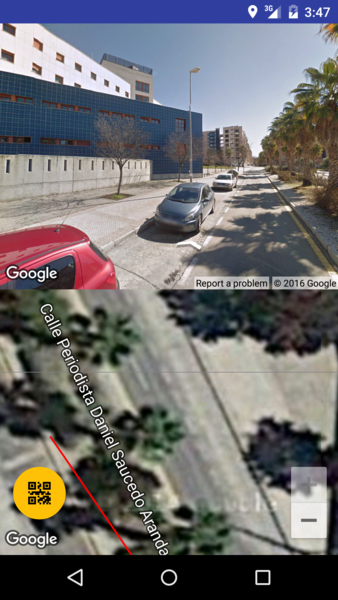
\includegraphics[width=0.5\textwidth]{./img/gpsQr.png}
\caption{GPSQR}
\end{figure}

El \emph{Floating Action Button} de abajo a la izquierda lanza el lector
de QRs, que usa una simplificación de la librería \emph{Zxing}. Cuando
se escanea una localización, veremos lo siguiente:

\begin{figure}[H]
\centering
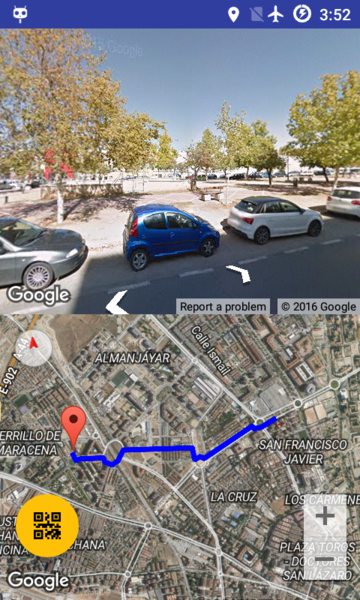
\includegraphics[width=0.5\textwidth]{./img/gqsqr_read.png}
\caption{Codigo QR leido con el destino}
\end{figure}

Una vez leido el QR, solo resta pulsar el marcador rojo para iniciar la
navegación con \emph{Google Maps}. La ruta calculada por la \emph{API}
de \emph{Google} es la azul, mientras que la ruta real tomada por el
usuario aparecerá en rojo.

\subsubsection{Implementación}\label{implementaciuxf3n-1}

Esta aplicación tiene dos clases, una para la primera y única pantalla y
otra es un servicio que se ejecuta en segundo plano, encargado de
obtener la localicación del usuario a un intervalo regular. Echemos
primero un vistazo al Servicio.

\paragraph{Clase
LocationUpdaterService.java}\label{clase-locationupdaterservice.java}

Extiende de \texttt{Service} e implementa las siguientes interfaces:

\begin{javacode}
	public class LocationUpdaterService extends Service implements
	        GoogleApiClient.ConnectionCallbacks,
	        GoogleApiClient.OnConnectionFailedListener,
	        LocationListener {
						// ....
					}
\end{javacode}

Con nombres bastantes descriptivos. Al iniciar el servicio, en su método
\texttt{onCreate} se construye el cliente para la API de google del
siguiente modo:

\begin{javacode}
	/**
	 * Builds a GoogleApiClient. Uses the {@code #addApi} method to request the
	 * LocationServices API.
	 */
	protected synchronized void buildGoogleApiClient() {
			if (BuildConfig.DEBUG) {
					Log.d(TAG, "Building GoogleApiClient");
			}
			mGoogleApiClient = new GoogleApiClient.Builder(this)
							.addConnectionCallbacks(this)
							.addOnConnectionFailedListener(this)
							.addApi(LocationServices.API)
							.build();
			createLocationRequest();
	}
\end{javacode}

También se inicializa el \texttt{BroadcastManager} que usaremos para
enviar las actualizaciones de la posición a la pantalla principal.

\begin{javacode}
mBroadcaster = LocalBroadcastManager.getInstance(this);
\end{javacode}

El método \texttt{onCreate} se llama una única vez, al crear el
servicio. Los comandos a ejecutar se colocan en el método
\texttt{onStartCommand}, este metodo lo crearemos como \emph{Sticky}, de
modo que si el sistema finaliza el proceso del servicio, se volverá a
ejecutar, volviendo así a obtener actualizaciones de localización:

\begin{javacode}
	@Override
	public int onStartCommand(Intent intent, int flags, int startId) {
			super.onStartCommand(intent, flags, startId);
			if (BuildConfig.DEBUG) {
					Log.d(TAG, "OnStartCommand");
			}

			if (mGoogleApiClient.isConnected()) {
				LocationServices.FusedLocationApi.requestLocationUpdates(mGoogleApiClient,
								mLocationRequest, this);
			}

			return START_STICKY;
	}
\end{javacode}

Una vez hecho esto, se llamarán a las interfaces implementadas con los
datos necesarios para obtener la localización actual, en este caso la
interfaz que nos interesa es \texttt{onLocationChanged}:

\begin{javacode}
	@Override
	public void onLocationChanged(Location location) {
			mCurrentLocation = location;
			mLastUpdateTime = DateFormat.getTimeInstance().format(new Date());
			sendResult(new LatLng(mCurrentLocation.getLatitude(), mCurrentLocation.getLongitude()));

			if (BuildConfig.DEBUG) {
					Log.d(TAG, mCurrentLocation.getLatitude() + ", " + mCurrentLocation.getLongitude());
			}
	}
\end{javacode}

El método \texttt{sendResult} se usa para emitir un \texttt{Broadcast}
al sistema y que la aplicación sea capaz de recibir el mensaje, incluso
si no está en primer plano:

\begin{javacode}
	/**
	 * This method send the current location to the activity who called the service, This way the
	 * location can be used in the UI.
	 *
	 * @param message The location
	 */
	private void sendResult(LatLng message) {
			Intent intent = new Intent(COPA_RESULT);
			if (message != null)
					intent.putExtra(COPA_MESSAGE, message);
			mBroadcaster.sendBroadcast(intent);
	}
\end{javacode}

Por último para que el Servicio funcione debemos registrarlo en el
\emph{Manifest} añadiendo la siguiente etiqueta:

\begin{xmlcode}
	<application>
		<!--//....-->
		<service android:name=".LocationUpdaterService"/>
		<!--//....-->
	</application>
\end{xmlcode}

\paragraph{Clase MapsActivity.java}\label{clase-mapsactivity.java}

Esta clase es la interfaz gráfica de la aplicación y donde se muestran
los dos mapas, para poder trabajar con ellos se implementan las
siguientes interfaces:

\begin{javacode}
	public class MapsActivity extends FragmentActivity implements
	        OnMapReadyCallback,
	        StreetViewPanorama.OnStreetViewPanoramaChangeListener,
	        OnStreetViewPanoramaReadyCallback {

				private GoogleMap mMap;
		    private StreetViewPanorama mStreetViewPanorama;

				// ...
	}
\end{javacode}

Antes de poder trabajar con cualquiera de los mapas hemos de esperar a
que estén inicializados, el momento de hacer esta inicialización es
cuando el sistema llama a \texttt{OnMapReadyCallback, OnStreetViewPanoramaReadyCallback}:

\begin{javacode}
	/**
	 * Manipulates the map once available.
	 * This callback is triggered when the map is ready to be used.
	 * This is where we can add markers or lines, add listeners or move the camera.
	 * If Google Play services is not installed on the device, the user will be prompted to install
	 * it inside the SupportMapFragment. This method will only be triggered once the user has
	 * installed Google Play services and returned to the app.
	 */
	@Override
	public void onMapReady(GoogleMap googleMap) {
			mMap = googleMap;
			mMap.setMapType(GoogleMap.MAP_TYPE_HYBRID);
			UiSettings uiSettings = mMap.getUiSettings();
			uiSettings.setMapToolbarEnabled(true);
			uiSettings.setZoomControlsEnabled(true);
	}

	@Override
	public void onStreetViewPanoramaReady(StreetViewPanorama panorama) {
			mStreetViewPanorama = panorama;
			mStreetViewPanorama.setOnStreetViewPanoramaChangeListener(this);
			mStreetViewPanorama.setStreetNamesEnabled(true);
	}
\end{javacode}

Entre otras cosas, en el método \texttt{onCreate} inicializamos el
\texttt{BroadcastReceiver} que nos permitirá recibir actualizaciones
desde el servicio, e iniciamos el servicio:

\begin{javacode}
	@Override
	protected void onCreate(final Bundle savedInstanceState) {
			super.onCreate(savedInstanceState);
			setContentView(R.layout.activity_maps);
	//  ...
			mLocationReceiver = new BroadcastReceiver() {
					@Override
					public void onReceive(Context context, Intent intent) {
							mPreviousLocation = mCurrentLocation;
							mCurrentLocation = intent.getParcelableExtra(LocationUpdaterService.COPA_MESSAGE);
							updateMap();
							mLocationsList.add(mCurrentLocation);

							if (BuildConfig.DEBUG) {
									Log.d(TAG, "LocationList size: " + mLocationsList.size());
							}
					}
			};

			mRequestLocationIntent = new Intent(this, LocationUpdaterService.class);
			startService(mRequestLocationIntent);
	// ...
	}
\end{javacode}

La función \texttt{updateMap} es la encargada de dibujar las líneas del
camino seguido por el usuario.

\subparagraph{Iniciar la navegación hasta
destino}\label{iniciar-la-navegaciuxf3n-hasta-destino}

Cuando se lanza el lector QR y se obtiene el destino, se crea una ruta a
seguir, en esta ruta es posible hacerla siguiendo el camino mostrado en
el mapa, o lanzando la navegación con \emph{Google Maps}. Para lo
último, es neceario pulsar sobre el marcador de destino y posteriormente
pulsar el icono de \emph{Google Maps}:

\begin{javacode}
	LatLng firstLocation = new LatLng(mCoord[0], mCoord[1]);
	mMap.addMarker(new MarkerOptions().position(firstLocation).title("Dest"));
	mMap.moveCamera(CameraUpdateFactory.newLatLng(firstLocation));
	mMap.animateCamera(CameraUpdateFactory.newLatLngZoom(firstLocation, 21.0f));

	GoogleDirection.withServerKey(getString(R.string.google_maps_server_key))
					.from(mCurrentLocation)
					.to(new LatLng(mCoord[0], mCoord[1]))
					.transportMode(TransportMode.WALKING)
					.execute(new DirectionCallback() {
							@Override
							public void onDirectionSuccess(Direction direction) {
									if (direction.isOK()) {
											Toast.makeText(getApplicationContext(), "DIRECTION KOK", Toast.LENGTH_LONG).show();
											ArrayList<LatLng> directionPositionList = direction.getRouteList().get(0).getLegList().get(0).getDirectionPoint();
											PolylineOptions polylineOptions = DirectionConverter.createPolyline(getApplicationContext(), directionPositionList, 5, Color.BLUE);
											mMap.addPolyline(polylineOptions);
									} else {
											Toast.makeText(getApplicationContext(), "NOT OK" + direction.getStatus(), Toast.LENGTH_LONG).show();
									}
							}

							@Override
							public void onDirectionFailure(Throwable t) {
									Toast.makeText(getApplicationContext(), "Failure", Toast.LENGTH_LONG).show();
							}
					});
\end{javacode}

\subparagraph{Permisos requeridos para el
AndroidManifest}\label{permisos-requeridos-para-el-androidmanifest-1}

\begin{xmlcode}
<uses-permission android:name="android.permission.ACCESS_FINE_LOCATION"/>
\end{xmlcode}

\subsubsection{Referencias y
agradecimientos}\label{referencias-y-agradecimientos}

\begin{itemize}
\itemsep1pt\parskip0pt\parsep0pt
\item
  \href{http://stackoverflow.com/a/14695943/1612432}{stackoverflow.com}
\item
  \href{https://github.com/googlesamples/android-play-location/tree/master/LocationUpdates}{github.com/googlesamples/android-play-location}
\item
  \href{https://github.com/akexorcist/Android-GoogleDirectionLibrary}{github.com/akexorcist/Android-GoogleDirectionLibrary}
\item
  \href{https://gist.github.com/blackcj/20efe2ac885c7297a676\#gistcomment-1666537}{gist.github.com/blackcj}
\item
  \href{https://github.com/googlemaps/android-samples}{github.com/googlemaps/android-samples}
\item
  \href{http://www.iconarchive.com/show/windows-8-icons-by-icons8/Ecommerce-Qr-Code-icon.html}{Icono
  QR}
\end{itemize}

\subsection{Photo Gesture}\label{photo-gesture}

Para realizar esta aplicación se ha usado una librería llamada
\href{https://github.com/DreaminginCodeZH/PatternLock}{PatterLock}.

En esta aplicación se le pide al usuario que establezca un patrón de
bloqueo, puede ser tan complejo como el patrón de bloqueo usado en
Android. Una vez establecido, cuando se introduzca correctamente la
aplicación tomará una foto a los 3 segundos. A continuación mostramos la
pantalla principal de la aplicación.

\begin{figure}[H]
\centering
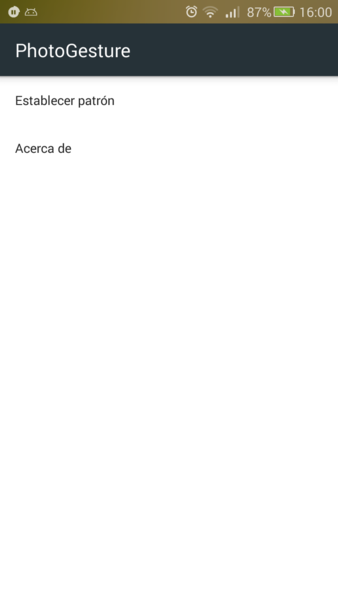
\includegraphics[width=0.5\textwidth]{./img/photoGesture.png}
\caption{Pantalla principal de photoGesture}
\end{figure}

Al pulsar \emph{``Establecer patrón''} veremos lo siguiente:

\begin{figure}[H]
\centering
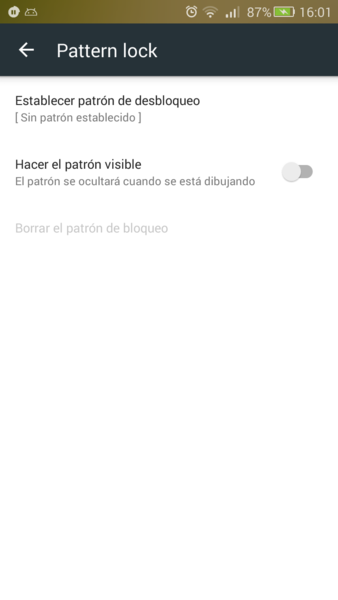
\includegraphics[width=0.5\textwidth]{./img/setPattern.png}
\caption{Establecer patrón}
\end{figure}

Es posible hacer que el patrón no sea visible cuando lo introducimos,
para añadir una capa extra de seguridad.

Cuando pulsemos \emph{Establecer patrón} se nos pedirá que lo dibujemos
dos veces, para confirmarlo:

\begin{figure}[H]
\centering
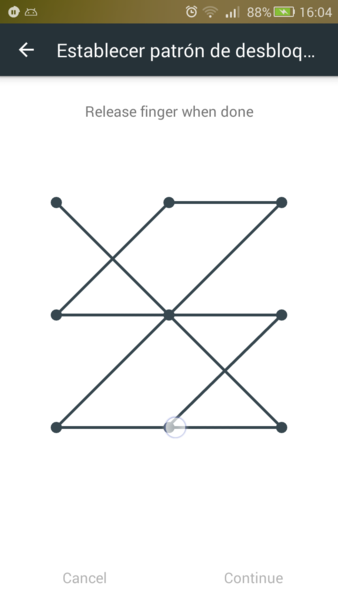
\includegraphics[width=0.5\textwidth]{./img/drawingPatter.png}
\caption{Dibujando el patrón}
\end{figure}

Hecho esto, cuando volvamos a la pantalla principal, en lugar de
``Establecer patrón'' aparecerá ``Echar foto''. Si pulsamos sobre ese
botón, se nos pide el patrón establecido. Si se introduce bien,
aparecerá la cámara con una cuenta atrás, al llegar a 0 se echará una
foto:

\begin{figure}[H]
\centering
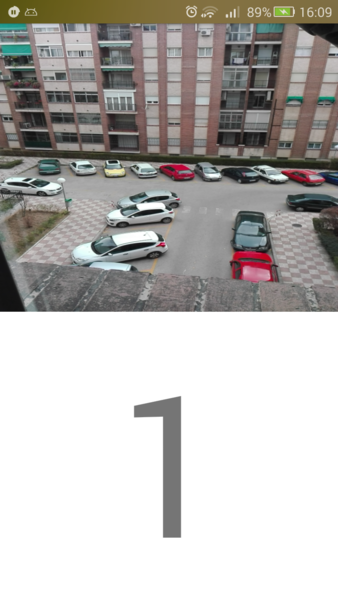
\includegraphics[width=0.5\textwidth]{./img/countdown.png}
\caption{Cuenta atrás para echar la foto}
\end{figure}

La foto se guardará en la galería.

\subsubsection{Implementación}\label{implementaciuxf3n-2}

Se ha reutilizado el ejemplo que el autor de la librería creo para
demostar su uso, y se ha modificado para ajustarlo a los requisitos de
la práctica. Para ello, cuando se introduce correctamente el parón, se
incia la actividad de hacer una foto:

\begin{javacode}
	@Override
	protected boolean isPatternCorrect(List<PatternView.Cell> pattern) {

			boolean isCorrect = PatternLockUtils.isPatternCorrect(pattern, this);
			if (isCorrect) {
					startActivity(new Intent(this, MakePhotoActivity.class));
			}

			return isCorrect;
	}
\end{javacode}

En la actividad \texttt{MakePhotoActivity} se muestra la pantalla
dividida en dos, arriba aparece la cámara y abajo una cuenta atrás de 3
segundos, cuando esta cuenta atrás llegue a cero, se hará la foto.

En el método \texttt{onCreate} se inicializa la cámara se crean dos
\emph{callbacks}, uno que se ejecuta al hacer la foto y otro para
reproducir un sonido al echar la foto:

\begin{javacode}
	mPicture = new Camera.PictureCallback() {

			@Override
			public void onPictureTaken(byte[] data, Camera camera) {

					File pictureFile = getOutputMediaFile(MEDIA_TYPE_IMAGE);
					if (pictureFile == null) {
							Log.e(TAG, "Error creating media file, check storage permissions: ");
							return;
					}

					try {
							FileOutputStream fos = new FileOutputStream(pictureFile);
							fos.write(data);
							fos.close();

							new MediaScannerWrapper(getApplicationContext(), pictureFile.getPath(), "image/jpeg").scan();
					} catch (FileNotFoundException e) {
							Log.d(TAG, "File not found: " + e.getMessage());
					} catch (IOException e) {
							Log.d(TAG, "Error accessing file: " + e.getMessage());
					}

			}
	};

	mShutterSound = MediaPlayer.create(this, R.raw.shut);

	mShutter = new Camera.ShutterCallback() {
			@Override
			public void onShutter() {
					mShutterSound.start();
					finish();
			}
	};
\end{javacode}

Al llegar la cuenta atrás a cero, se llama al método
\texttt{takePicture} de la cámara y se le pasan los \emph{callbacks
anteriores}:

\begin{javacode}
mCamera.takePicture(mShutter, null, mPicture);
\end{javacode}

\subparagraph{Mostrando una vista previa de la
cámara}\label{mostrando-una-vista-previa-de-la-cuxe1mara}

Para crear la parte superior de la pantalla, en la que se muestra una
vista previa de la cámara, hay que crear una clase extendiendo de
\texttt{SurfaceView} que hemos llamado \texttt{CameraPreview}, esta
clase implementa la interfaz \texttt{SurfaceHolder.Callback}:

\begin{javacode}
	/** A basic Camera preview class */
	public class CameraPreview extends SurfaceView implements SurfaceHolder.Callback {

	    private SurfaceHolder mHolder;
	    private Camera mCamera;

	    public CameraPreview(Context context, Camera camera) {
	        super(context);
	        mCamera = camera;

	        mCamera.setDisplayOrientation(90);
	        // Install a SurfaceHolder.Callback so we get notified when the
	        // underlying surface is created and destroyed.
	        mHolder = getHolder();
	        mHolder.addCallback(this);
	        // deprecated setting, but required on Android versions prior to 3.0
	        mHolder.setType(SurfaceHolder.SURFACE_TYPE_PUSH_BUFFERS);
	    }

	    public void surfaceCreated(SurfaceHolder holder) {
	        // The Surface has been created, now tell the camera where to draw the preview.
	        try {
	            mCamera.setPreviewDisplay(holder);
	            mCamera.startPreview();
	        } catch (IOException e) {
	            Log.d("TAG", "Error setting camera preview: " + e.getMessage());
	        }
	    }

	    public void surfaceDestroyed(SurfaceHolder holder) {
	        // empty. Take care of releasing the Camera preview in your activity.
	        mCamera.release();
	    }

	    public void surfaceChanged(SurfaceHolder holder, int format, int w, int h) {
	        // If your preview can change or rotate, take care of those events here.
	        // Make sure to stop the preview before resizing or reformatting it.

	        if (mHolder.getSurface() == null) {
	            // preview surface does not exist
	            return;
	        }

	        // stop preview before making changes
	        try {
	            mCamera.stopPreview();
	        } catch (Exception e) {
	            // ignore: tried to stop a non-existent preview
	        }

	        // set preview size and make any resize, rotate or
	        // reformatting changes here

	        // start preview with new settings
	        try {
	            mCamera.setPreviewDisplay(mHolder);
	            mCamera.startPreview();

	        } catch (Exception e) {
	            Log.d("TAG", "Error starting camera preview: " + e.getMessage());
	        }
	    }
	}
\end{javacode}

\subparagraph{Permisos requeridos para el
AndroidManifest}\label{permisos-requeridos-para-el-androidmanifest-2}

\begin{xmlcode}
	<uses-permission android:name="android.permission.CAMERA" />
	<uses-permission android:name="android.permission.WRITE_EXTERNAL_STORAGE" />
\end{xmlcode}

\subsubsection{Referencias}\label{referencias-1}

\begin{itemize}
\itemsep1pt\parskip0pt\parsep0pt
\item
  Página oficial de Android \textbar{}
  \href{http://developer.android.com/guide/topics/media/camera.html}{developer.android.com/guide/topics/media/camera}
\item
  Librería PatternLock \textbar{}
  \href{https://github.com/DreaminginCodeZH/PatternLock}{github.com/DreaminginCodeZH/PatternLock}
\end{itemize}

\subsection{Movement Sound}\label{movement-sound}

En esta aplicación se usa el acelerómetro y el giroscopio, para mostrar
sus valores por pantalla. El giroscopio es capaz de detectar una
rotación del dispositivo, al hacerlo, reproduce un sonido. Por contra,
el acelerómetro detecta una sacudida del dispositivo y reproduce un
sonido distinto. Debido a que no en todos los dispositivos se obtienen
valores precisos para los sensores, solo se mostrarán aquellos que
tengan sentido.

\begin{figure}[H]
\centering
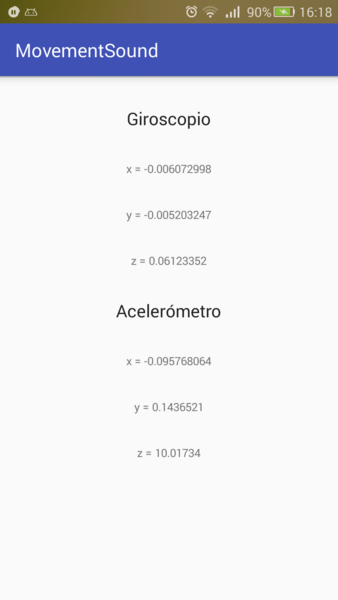
\includegraphics[width=0.5\textwidth]{./img/movementSound.png}
\caption{Aplicación Movement Sound}
\end{figure}

\subsubsection{Implementación}\label{implementaciuxf3n-3}

\paragraph{Para instanciar ambos sensores en el
\texttt{onCreate}:}\label{para-instanciar-ambos-sensores-en-el-oncreate}

\begin{javacode}
	// Get the sensors to use
	mSensorManager = (SensorManager) getSystemService(Context.SENSOR_SERVICE);
	mSensorAcc = mSensorManager.getDefaultSensor(Sensor.TYPE_ACCELEROMETER);
	mSensorGyr = mSensorManager.getDefaultSensor(Sensor.TYPE_GYROSCOPE);
\end{javacode}

Cuando el tengamos datos nuevos de los sensores, los actualizaremos en
el \texttt{onSensorChanged}:

\begin{javacode}
	@Override
	public void onSensorChanged(SensorEvent event) {

			if (event.accuracy == SensorManager.SENSOR_STATUS_UNRELIABLE) {

					if (event.sensor.getType() == Sensor.TYPE_ACCELEROMETER) {
							mAccx.setText(R.string.act_main_no_acuracy);
							mAccy.setText(R.string.act_main_no_acuracy);
							mAccz.setText(R.string.act_main_no_acuracy);
					} else if (event.sensor.getType() == Sensor.TYPE_GYROSCOPE) {
							mGyrox.setText(R.string.act_main_no_acuracy);
							mGyroy.setText(R.string.act_main_no_acuracy);
							mGyroz.setText(R.string.act_main_no_acuracy);
					}
					return;
			}

			if (event.sensor.getType() == Sensor.TYPE_ACCELEROMETER) {
					mAccx.setText("x = " + Float.toString(event.values[0]));
					mAccy.setText("y = " + Float.toString(event.values[1]));
					mAccz.setText("z = " + Float.toString(event.values[2]));
					detectShake(event);
			} else if (event.sensor.getType() == Sensor.TYPE_GYROSCOPE) {
					mGyrox.setText("x = " + Float.toString(event.values[0]));
					mGyroy.setText("y = " + Float.toString(event.values[1]));
					mGyroz.setText("z = " + Float.toString(event.values[2]));
					detectRotation(event);
			}

	}
\end{javacode}

Si el acelerómetro está activo, se intentará detectar una sacudida del
dispositivo y se reproducirá un sonido, en el caso del giroscopio, se
pretende detectar una rotación del dispositivo. Estos patrones se
reconocen con las siguientes funciones:

\begin{javacode}
	// References:
	//  - http://jasonmcreynolds.com/?p=388
	//  - http://code.tutsplus.com/tutorials/using-the-accelerometer-on-android--mobile-22125

	/**
	 * Detect a shake based on the ACCELEROMETER sensor
	 *
	 * @param event
	 */
	private void detectShake(SensorEvent event) {
			long now = System.currentTimeMillis();

			if ((now - mShakeTime) > SHAKE_WAIT_TIME_MS) {
					mShakeTime = now;

					float gX = event.values[0] / SensorManager.GRAVITY_EARTH;
					float gY = event.values[1] / SensorManager.GRAVITY_EARTH;
					float gZ = event.values[2] / SensorManager.GRAVITY_EARTH;

					// gForce will be close to 1 when there is no movement
					double gForce = Math.sqrt(gX * gX + gY * gY + gZ * gZ);

					// Change background color if gForce exceeds threshold;
					// otherwise, reset the color
					if (gForce > SHAKE_THRESHOLD) {
							soundAcc.start();
					}
			}
	}

	/**
	 * Detect a rotation in on the GYROSCOPE sensor
	 *
	 * @param event
	 */
	private void detectRotation(SensorEvent event) {
			long now = System.currentTimeMillis();

			if ((now - mRotationTime) > ROTATION_WAIT_TIME_MS) {
					mRotationTime = now;

					// Change background color if rate of rotation around any
					// axis and in any direction exceeds threshold;
					// otherwise, reset the color
					if (Math.abs(event.values[0]) > ROTATION_THRESHOLD ||
									Math.abs(event.values[1]) > ROTATION_THRESHOLD ||
									Math.abs(event.values[2]) > ROTATION_THRESHOLD) {
							soundGyro.start();
					}
			}
	}
\end{javacode}

\subparagraph{Permisos requeridos para el
AndroidManifest}\label{permisos-requeridos-para-el-androidmanifest-3}

\begin{xmlcode}
	<uses-permission android:name="android.hardware.sensor.gyroscope"/>
	<uses-permission android:name="android.hardware.sensor.accelerometer"/>
\end{xmlcode}

\subsubsection{Referencias}\label{referencias-2}

\begin{itemize}
\itemsep1pt\parskip0pt\parsep0pt
\item
  AndroidWearMotionSensors \textbar{}
  \href{https://github.com/drejkim/AndroidWearMotionSensors}{github.com/drejkim}
\end{itemize}


\end{document}
